%=======================================================
% usepackage
\usepackage{latexsym}
\usepackage{amssymb}
\usepackage{amsthm}
\usepackage{amscd}
\usepackage{amsmath}
\usepackage{mathrsfs}
\usepackage{graphicx}
\usepackage{hyperref}
\usepackage{shuffle}
\usepackage{stmaryrd}
\usepackage{enumitem}
\usepackage[noabbrev]{cleveref}
\usepackage{ytableau}

\newcommand\crefrangeconjunction{\textendash}


%\usepackage[all]{xy}
%\input xy \xyoption{frame}
%\xyoption{dvips}
%\UseCrayolaColors

\usepackage[colorinlistoftodos]{todonotes}
\usetikzlibrary{chains,scopes,decorations.markings}

\usepackage{tikz-cd}

%=========================================================================
% theorem declarations
\theoremstyle{definition}
\newtheorem* {theorem*}{Theorem}
\newtheorem* {conjecture*}{Conjecture}
\newtheorem{theorem}{Theorem}[section]
\newtheorem{thmdef}[theorem]{Theorem-Definition}
\newtheorem{propdef}[theorem]{Proposition-Definition}
\newtheorem{question}[theorem]{Question}
\theoremstyle{definition}
\newtheorem{observation}[theorem]{Observation}
\newtheorem {claim}{Claim}
\newtheorem* {example*}{Example}
\newtheorem* {fact}{Fact}
\newtheorem{lemma}[theorem]{Lemma}
\theoremstyle{definition}
\newtheorem{definition}[theorem]{Definition}
\theoremstyle{definition}
\newtheorem* {notation}{Notation}
\newtheorem{conjecture}[theorem]{Conjecture}
\newtheorem{proposition}[theorem]{Proposition}
\newtheorem{corollary}[theorem]{Corollary}
\newtheorem{algorithm}[theorem]{Algorithm}
\newtheorem* {remark*}{Remark}
\newtheorem{remark}[theorem]{Remark}
\theoremstyle{definition}
\newtheorem {example}[theorem]{Example}
\theoremstyle{definition}
\newtheorem* {examples}{Examples}
\theoremstyle{definition}
\newtheorem* {exercise}{Exercise}
\theoremstyle{definition}
\newtheorem{problem}[theorem]{Problem}
\theoremstyle{definition}
\newtheorem* {remarks}{Remarks}



\newcommand{\Fl}{\operatorname{Fl}}
\newcommand{\std}{\operatorname{std}}
\newcommand{\Proj}{\operatorname{Proj}}
\newcommand{\dist}{\operatorname{dist}}
\newcommand{\Des}{\operatorname{Des}}
\newcommand{\DesR}{\operatorname{Des}_R}
\newcommand{\DesL}{\operatorname{Des}_L}
\newcommand{\im}{\operatorname{im}}
\newcommand{\supp}{\operatorname{supp}}
\newcommand{\Inv}{\mathrm{Inv}}
\newcommand{\Ess}{\operatorname{Ess}}
\newcommand{\rank}{\operatorname{rank}}
\renewcommand{\dim}{\operatorname{dim}}
\newcommand{\DesV}{\operatorname{Des}_V}
\newcommand{\Asc}{\operatorname{Asc}}
\newcommand{\asc}{\operatorname{asc}}
\newcommand{\des}{\operatorname{des}}
\newcommand{\last}{\operatorname{end}}
\newcommand{\shift}{\operatorname{shift}}



\newcommand{\modu}{\ (\mathrm{mod}\ }
\renewcommand{\(}{\left(}
\renewcommand{\)}{\right)}
\newcommand{\sP}{\mathscr{P}}
\newcommand{\FF}{\mathbb{F}}
\newcommand{\CC}{\mathbb{C}}
\newcommand{\QQ}{\mathbb{Q}}
\newcommand{\cP}{\mathcal{P}}
\newcommand{\cQ}{\mathcal{Q}}
\newcommand{\cK}{\mathcal{K}}
\newcommand{\cR}{\mathcal{R}}
\newcommand{\V}{\mathcal{V}}
\newcommand{\cS}{\mathcal{S}}
\newcommand{\cI}{\mathcal{I}}
\newcommand{\cJ}{\mathcal{J}}
\newcommand{\cC}{\mathcal{C}}
\newcommand{\cD}{\mathcal{D}}
\newcommand{\cZ}{\mathcal{Z}}
\newcommand{\cX}{\mathcal{X}}
\newcommand{\cW}{\mathcal{W}}
\newcommand{\cY}{\mathcal{Y}}

\newcommand{\tr}{\mathrm{tr}}
\newcommand{\Hom}{\mathrm{Hom}}
\newcommand{\End}{\mathrm{End}}
\newcommand{\RR}{\mathbb{R}}
\newcommand{\ZZ}{\mathbb{Z}}
\newcommand{\Aut}{\mathrm{Aut}}


\newcommand{\spanning}{\textnormal{-span}} 
\newcommand{\cyc}{\textsf{cyc}}



\newcommand{\fkn}{\mathfrak{n}}

\newcommand{\cM}{\mathcal{M}}
\newcommand{\cN}{\mathcal{N}}
\newcommand{\cL}{\mathcal{L}}
\newcommand{\g}{\mathfrak{g}}
\newcommand{\One}{{1\hspace{-.15.5cm} 1}}
\newcommand{\one}{{1\hspace{-.11cm} 1}}

\newcommand{\sgn}{\mathrm{sgn}}
\newcommand{\fka}{\mathfrak{a}}
\newcommand{\fkh}{\mathfrak{h}}



\newcommand{\fk}{\mathfrak}

\newcommand{\barr}{\begin{array}}
\newcommand{\earr}{\end{array}}
\newcommand{\ba}{\begin{aligned}}
\newcommand{\ea}{\end{aligned}}
\newcommand{\be}{\begin{equation}}
\newcommand{\ee}{\end{equation}}

\newcommand{\Cyc}{\mathrm{Cyc}}
\newcommand{\Fix}{\mathrm{Fix}}
\newcommand{\Pair}{\mathrm{Pair}}
\newcommand{\pair}{\mathrm{pair}}

\newcommand{\qquand}{\qquad\text{and}\qquad}
\newcommand{\quand}{\quad\text{and}\quad}
\newcommand{\qquord}{\qquad\text{or}\qquad}
\newcommand{\quord}{\quad\text{or}\quad}

\newcommand{\gl}{\mathfrak{gl}}






\newcommand{\I}{\mathsf{Invol}}
\newcommand{\Invol}{I_n}
\newcommand{\Ivex}{I^{\mathsf{vex}}_n}
\newcommand{\cH}{\mathcal H}






\newcommand{\ds}{\displaystyle}

\newcommand{\proj}{\mathrm{proj}}

\newcommand{\id}{\mathrm{id}}

\newcommand{\PP}{\mathbb{Z}_{>0}}
\newcommand{\NN}{\mathbb{Z}_{\geq 0}}



\newcommand{\fkS}{\fk S}



\newcommand{\ben}{\begin{enumerate}}
\newcommand{\een}{\end{enumerate}}

\newcommand{\bei}{\begin{itemize}}
\newcommand{\eei}{\end{itemize}}

\newcommand{\cT}{\mathscr{T}}
\newcommand{\sU}{\mathscr{U}}
\newcommand{\cE}{\mathcal E}
\newcommand{\invol}{\textbf{invol}}

\newcommand{\Mon}[1]{\mathscr{F}(#1)}










\newcommand{\xRightarrow}[2][]{\ext@arrow 0359\Rightarrowfill@{#1}{#2}}




\newcommand{\Sp}{\mathsf{Sp}}





\renewcommand{\r}[1]{\textcolor{red}{#1}}



\newcommand{\cA}{\mathcal{A}}
\newcommand{\cB}{\mathcal{B}}
\newcommand{\iB}{\hat\cB}
\newcommand{\fB}{\hat\cB^\fpf}
















\newcommand{\cG}{\mathcal{G}}














\renewcommand{\bar}{\overline}














\newcommand{\Clans}{\mathsf{Clans}}
\newcommand{\D}{\mathsf{D}}


\definecolor{darkred}{rgb}{0.7,0,0} % darkred color
\newcommand{\defn}[1]{{\color{darkred}\emph{#1}}} % emphasis of a definition



\newcommand{\Sym}{\mathsf{Sym}}
\newcommand{\QSym}{\mathsf{QSym}}


\newcommand{\op}{\mathsf{op}}


\usepackage{pbox}
\tikzset{every loop/.style={min distance=10 mm, in=60, out=120, looseness=10}}
\tikzset{
dot/.style = {circle, fill, inner sep=2.2,outer sep=0},
% dot/.default = 6pt % size of the circle diameter 
}



\numberwithin{equation}{section}
\allowdisplaybreaks[1]



\newcommand{\arxiv}[1]{\href{https://arxiv.org/abs/#1}{\texttt{arXiv:#1}}}



\newcommand{\bpartial}{\partial^{(\beta)}}

\newcommand{\fkGO}{\mathfrak{G}^{\mathsf{O}}}

\newcommand{\MX}{M\hspace{-0.5mm}X}
\newcommand{\Mat}{\mathsf{Mat}}
\newcommand{\codim}{\mathrm{codim}}




\newcommand{\iG}{\widehat{\cG}}
\newcommand{\cU}{\mathcal{U}}
\newcommand{\SD}{\mathsf{SD}}







\newcommand{\word}{\mathsf{word}}


\newcommand{\iD}{\hat D}

\newcommand{\ellinv}{\ell_{\mathsf{inv}}}



\newcommand{\NW}{\mathsf{NW}}
\newcommand{\alignNW}{\mathrm{align}_{\NW}}

\newcommand{\bff}{\mathbf{f}}

\newcommand{\ytabc}[2]{
\ytableausetup{boxsize = #1,aligntableaux=center}
{\begin{ytableau}  #2  \end{ytableau}}
}




\usepackage{nicematrix}
\usepackage{mathtools}
\usepackage{verbatim}

\newcommand{\sdgap}{ \\[-4pt]\\ }

\newcommand{\symDef}{\mathsf{symDef}}
\newcommand{\cWsim}{\sim_\cW}
\newcommand{\fkG}{\mathfrak{G}^{(\beta)}}
\renewcommand{\iG}{\widehat{\mathfrak{G}}^{(\beta)}}

\newcommand{\SPP}{\mathsf{ShPP}}
\newcommand{\SetSPP}{\mathsf{SetShPP}}
\newcommand{\SetPP}{\mathsf{SetPP}}

\newcommand{\MPipes}{\mathsf{MPipes}}


\newcommand{\invRothe}{\mathsf{invRothe}}
\newcommand{\double}{\mathsf{double}}
\newcommand{\halve}{\mathsf{halve}}
\newcommand{\transpose}{\mathsf{transpose}}


\newcommand{\GPD}{\mathsf{GPD}}
\newcommand{\BPD}{\mathsf{BPD}}

\newcommand{\kGPD}{\mathsf{GPD}_K}
\newcommand{\kBPD}{\mathsf{BPD}_K}

\newcommand{\InvPD}{\mathsf{InvGPD}}
\newcommand{\InvGPD}{\InvPD}
\newcommand{\InvBPD}{\mathsf{InvBPD}}
\newcommand{\MInvBPD}{\mathsf{InvMBPD}}

\newcommand{\kInvPD}{\mathsf{InvGPD}_K}
\newcommand{\kInvBPD}{\mathsf{InvBPD}_K}

\newcommand{\kweight}{\weight_K}
\newcommand{\hatkweight}{\widehat\weight_K}
\newcommand{\kpi}{\overline{\pi}}
\newcommand{\kzeta}{\overline{\zeta}}


\newcommand{\NRes}{\mathrm{NRes}}
\newcommand{\NDes}{\mathrm{NDes}}


\newcommand{\circled}[1]{\text{\textcircled{\raisebox{-0.9pt}{#1}}}}



\newcommand{\symDroop}{\mathsf{symDroop}}
\newcommand{\complexDroop}{\mathsf{complexDroop}}
\newcommand{\droop}{\mathsf{droop}}
\newcommand{\kdroop}{\mathsf{kDroop}}

\newcommand{\extComplexDroop}{\mathsf{strongComplexDroop}}
\newcommand{\extDroop}{\mathsf{strongDroop}}

\newcommand{\undroop}{\mathsf{undroop}}
\newcommand{\complexUndroop}{\mathsf{complexUndroop}}

\newcommand{\bend}{\mathsf{bend}}

\newcommand{\iS}{\widehat{\fkS}}
\newcommand{\half}{\mathsf{half}}
\renewcommand{\cP}{\mathsf{BPD}}
\newcommand{\cRP}{\mathsf{RBPD}}

\newcommand{\SymRP}{\mathsf{SymBPD}}
\newcommand{\iRP}{\mathsf{InvBPD}}

\newcommand{\weight}{\mathsf{wt}}

\newcommand{\blank}{\mathsf{blank}}
\newcommand{\cross}{\mathsf{cross}}
\newcommand{\bump}{\mathsf{bump}}
\newcommand{\upturn}{\mathsf{upturn}}
\newcommand{\rothe}{\mathsf{rothe}}

\newcommand{\NCwest}{\mathcal{C}_{\mathrm{west}}}
\newcommand{\NCsouth}{\mathcal{C}_{\mathrm{south}}}
\newcommand{\NCnorth}{\mathcal{C}_{\mathrm{north}}}
\newcommand{\NCeast}{\mathcal{C}_{\mathrm{east}}}
\newcommand{\NCdiag}{\mathcal{C}_{\mathrm{diag}}}
\renewcommand{\std}[2]{#1\cap #2}

\newcommand{\ASM}{\mathrm{ASM}}
\newcommand{\DASM}{\mathrm{DASM}}
\newcommand{\wt}{\mathrm{wt}}
\newcommand{\hatu}{\widehat{u}}
\newcommand{\uPrime}{\ell}
\newcommand{\hatuPrime}{\widehat{\ell}}
\newcommand{\diag}{\mathrm{diag}}


\newcommand{\cTGPD}{\cT_{\mathsf{GPD}}}

\newcommand{\cToff}{\cT_{\mathrm{off}}}
\newcommand{\cTdiag}{\cT_{\mathrm{diag}}}

\newcommand{\flatten}{\mathsf{flatten}}


\newcommand{\cJdiag}{\mathcal{J}_{\Delta}}
\newcommand{\cJoff}{\mathcal{J}}
\newcommand{\cBdiag}{\mathcal{B}_{\Delta}}
\newcommand{\cBoff}{\mathcal{B}}

\newcommand{\cJBdiag}{\mathcal{M}_\Delta}





\newcommand{\init}{\mathrm{init}}
\newcommand{\mon}{\mathbf{m}}
\newcommand{\SymMat}{\Mat^{\mathrm{sym}}}
\newcommand{\MSV}{\mathsf{MSV}}
\newcommand{\SymMSV}{\MSV^{\mathrm{sym}}}
\newcommand{\SymI}{I^{\mathrm{sym}}}
\newcommand{\SymJ}{J^{\mathrm{sym}}}
\newcommand{\cSymG}{\cG^{\mathrm{sym}}}
\newcommand{\mat}[1]{\left[ \begin{array} #1 \end{array}\right]}
\renewcommand{\vec}[1]{\mat{{r} #1}}

\newcommand{\UT}{\nabla}
\newcommand{\LT}{\mathsf{LT}}

%\newcommand{\UT}{\raisebox{-0.5pt}{\tikz{\draw (.25,.25) -- (.25,0) -- (0,.25) -- (.25,.25);}}\hspace{0.5pt}}

%\renewcommand{\LT}{\raisebox{-0.5pt}{\tikz{\draw (0,0) -- (.25,0) -- (0,.25) -- (0,0);}}\hspace{0.5pt}}

\newcommand{\displace}{\mathsf{displace}}
\newcommand{\SymDelta}{\Delta^{\mathrm{sym}}}
\newcommand{\iGconj}{\widetilde{\mathfrak{G}}^{\textsf{O}}}
\newcommand{\link}{\mathrm{lk}}


\newcommand{\DBox}{D^{\mathsf{dbl}}}
\newcommand{\bft}{\mathbf t}
\newcommand{\bftrev}{\bft^{\mathsf{rev}}}
\newcommand{\calT}{\mathcal{T}}
\newcommand{\CaseA}{Case (A)}
\newcommand{\CaseB}{Case (B)}
\newcommand{\CaseC}{Case (C)}

%\newcommand{\VInv}{\operatorname{VInv}}
\newcommand{\bpdwidth}{1.2em}
\newcommand{\bpdsmallwidth}{1.0em}

\newcommand{\ETILE}{
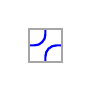
\begin{tikzpicture}[x=\bpdwidth,y=\bpdwidth,baseline=(z.base)]
\node at (0.5,1.25) (z) {};
\draw[thick,rounded corners,color=blue] (.5,2)--(.5,1.5)--(0,1.5);
\draw[thick,rounded corners,color=blue] (.5,1)--(.5,1.5)--(1,1.5);
\draw[gray!70, line width=0.7pt](0,1)rectangle(1,2);
\end{tikzpicture}
}

\newcommand{\JTILE}{
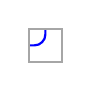
\begin{tikzpicture}[x=\bpdwidth,y=\bpdwidth,baseline=(z.base)]
\node at (0.5,1.25) (z) {};
\draw[thick,rounded corners,color=blue] (.5,2)--(.5,1.5)--(0,1.5);
\draw[gray!70, line width=0.7pt](0,1)rectangle(1,2);
\end{tikzpicture}
}

\newcommand{\CTILE}{
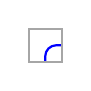
\begin{tikzpicture}[x=\bpdwidth,y=\bpdwidth,baseline=(z.base)]
\node at (0.5,1.25) (z) {};
\draw[thick,rounded corners,color=blue] (.5,1)--(.5,1.5)--(1,1.5);
\draw[gray!70, line width=0.7pt](0,1)rectangle(1,2);
\end{tikzpicture}
}

\newcommand{\PTILE}{
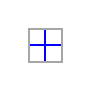
\begin{tikzpicture}[x=\bpdwidth,y=\bpdwidth,baseline=(z.base)]
\node at (0.5,1.25) (z) {};
\draw[thick,rounded corners,color=blue] (0,1.5)--(1,1.5);
\draw[thick,rounded corners,color=blue] (.5,1)--(.5,2);
\draw[gray!70, line width=0.7pt](0,1)rectangle(1,2);
\end{tikzpicture}
}

\newcommand{\HTILE}{

\begin{tikzpicture}[x=\bpdwidth,y=\bpdwidth,baseline=(z.base)]
\node at (0.5,1.25) (z) {};
\draw[thick,rounded corners,color=blue] (0,1.5)--(1,1.5);
\draw[gray!70, line width=0.7pt](0,1)rectangle(1,2);
\end{tikzpicture}
}

\newcommand{\VTILE}{

\begin{tikzpicture}[x=\bpdwidth,y=\bpdwidth,baseline=(z.base)]
\node at (0.5,1.25) (z) {};
\draw[thick,rounded corners,color=blue] (.5,1)--(.5,2);
\draw[gray!70, line width=0.7pt](0,1)rectangle(1,2);
\end{tikzpicture}}

\newcommand{\BTILE}{

\begin{tikzpicture}[x=\bpdwidth,y=\bpdwidth,baseline=(z.base)]
\node at (0.5,1.25) (z) {};
\draw[gray!70, line width=0.7pt](0,1)rectangle(1,2);
\end{tikzpicture}
}



\newcommand{\JDIAG}{

\begin{tikzpicture}[x=\bpdwidth,y=\bpdwidth,baseline=(z.base)]
\node at (0.5,1.25) (z) {};
\draw[thick,rounded corners,color=blue] (.5,1.5)--(0,1.5);
\draw[white, line width=0.7pt,fill=white] (1,2)--(1,1)--(0,2)--(1,2);
\draw[gray!70, line width=0.7pt] (0,1)--(1,1)--(0,2)--(0,1);
\end{tikzpicture}
}

\newcommand{\CDIAG}{

\begin{tikzpicture}[x=\bpdwidth,y=\bpdwidth,baseline=(z.base)]
\node at (0.5,1.25) (z) {};
\draw[thick,rounded corners,color=blue] (.5,1)--(.5,1.5);
\draw[white, line width=0.7pt,fill=white] (1,2)--(1,1)--(0,2)--(1,2);
\draw[gray!70, line width=0.7pt] (0,1)--(1,1)--(0,2)--(0,1);
\end{tikzpicture}
}

\newcommand{\PDIAG}{
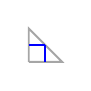
\begin{tikzpicture}[x=\bpdwidth,y=\bpdwidth,baseline=(z.base)]
\node at (0.5,1.25) (z) {};
%\draw[thick,rounded corners,color=blue] (0,1.5)--(1,1.5);
%\draw[thick,rounded corners,color=blue] (.5,1)--(.5,2);
\draw[white, line width=0.7pt,fill=white] (1,2)--(1,1)--(0,2)--(1,2);
\draw[gray!70, line width=0.7pt] (0,1)--(1,1)--(0,2)--(0,1);
\draw[thick,rounded corners,color=blue] (0,1.5)--(0.5,1.5);
\draw[thick,rounded corners,color=blue] (.5,1)--(.5,1.5);
\end{tikzpicture}
}

\newcommand{\BDIAG}{

\begin{tikzpicture}[x=\bpdwidth,y=\bpdwidth,baseline=(z.base)]
\node at (0.5,1.25) (z) {};
\draw[white, line width=0.7pt,fill=white] (1,2)--(1,1)--(0,2)--(1,2);
\draw[gray!70, line width=0.7pt] (0,1)--(1,1)--(0,2)--(0,1);
\end{tikzpicture}
}

\newcommand{\EDIAG}{
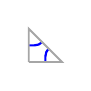
\begin{tikzpicture}[x=\bpdwidth,y=\bpdwidth,baseline=(z.base)]
\node at (0.5,1.25) (z) {};
\draw[thick,rounded corners,color=blue] (.5,2)--(.5,1.5)--(0,1.5);
\draw[thick,rounded corners,color=blue] (.5,1)--(.5,1.5)--(1,1.5);
\draw[white, line width=0.7pt,fill=white] (1,2)--(1,1)--(0,2)--(1,2);
\draw[gray!70, line width=0.7pt] (0,1)--(1,1)--(0,2)--(0,1);
\end{tikzpicture}
}


\DeclareMathOperator{\MD}{MD}
\DeclareMathOperator{\BZOD}{BZOD}
\DeclareMathOperator{\MOD}{MOD}
%\DeclareMathOperator{\DASM}{DASM}
%\DeclareMathOperator{\ASM}{ASM}



\newcommand{\eric}[1]{\todo[inline,size=\tiny,color=green!30]{#1 \\ \hfill --- E.}}
\newcommand{\Eric}[1]{\todo[size=\tiny,color=green!30]{#1 \\ \hfill --- E.}}


\newcommand{\alejandro}[1]{\todo[inline,size=\tiny,color=blue!30]{#1 \\ \hfill --- A.}}
\newcommand{\Alejandro}[1]{\todo[size=\tiny,color=blue!30]{#1 \\ \hfill --- A.}}

\newcommand{\tianyi}[1]{\todo[inline,size=\tiny,color=red!30]{#1 \\ \hfill --- T.}}
\newcommand{\Tianyi}[1]{\todo[size=\tiny,color=red!30]{#1 \\ \hfill --- T.}}






\newcommand{\fkSO}{\fkS^{\mathsf{O}}}
 \renewcommand{\O}{\mathsf{O}}
 \newcommand{\inv}{\mathrm{inv}}


\newtheorem{mainthm}{Theorem}
\renewcommand{\themainthm}{\Alph{mainthm}}